\chapter{Downsampling and upsampling images}

Sampling is also an important linear operation when working with discrete images. Many times we will be interested in changing the resolution of a discrete image by going down or up in resolution. Going down in resolution (downsampling) is done by dropping samples and going up in resolution (upsampling) requires adding new samples by interpolation. In both cases, it is important to understand what happens with the signal in order to avoid introducing undesired distortions in the image. We will use these two operations many times in this and the following chapters. 

In the previous chapter we discussed the case when the input is a continuous signal and the output is its discretized version. The analysis we will do here is very similar to the one in the previous chapter. 

\section{Downsampling}

Downsampling an image of size $N \times M$ by a factor of $k$, where $N$ and $M$ are divisible by $k$, results in a lower resolution image of size $N/k \times M/k$. We will use the following notation:
\begin{equation}
f_{\downarrow k} \left[n,m\right]   = f\left[n,m\right] \downarrow k = f\left[kn,km\right]
\end{equation}

\marginnote{Downsampling is often drawn using the following block:
~\\
%\begin{figure}[h!]
\begin{center}
\tikzstyle{int}=[draw, minimum size=3em]
\tikzstyle{init} = [pin edge={to-,thin,black}]
\begin{tikzpicture}[node distance=0cm,auto,>=latex']
  \node [int] (box1) {$\downarrow k$};
   \node [left of=box1,node distance=1.1cm] (input) {$f $};
   \node [right of=box1,node distance=1.4cm] (output) {$f_{\downarrow k}$};
    \node (c) [right of=box1,node distance=3cm, coordinate] {};
    \path[->] (input) edge node {} (box1);
    \path[->] (box1) edge node {} (output);
\end{tikzpicture}
\end{center}
%\label{fig:genericfilterH}
%\end{figure}
}

Downsampling is a linear operation. In the 1D case, for a signal of length 8, subsampling by a factor of 2 can be described by the following linear operator:
\begin{equation}
D = \left[ 
\begin{array}{cccccccc}
1 & 0 & 0 & 0 & 0 & 0 & 0 & 0\\
0 & 0 & 1 & 0 & 0 & 0 & 0 & 0\\
0 & 0 & 0 & 0 & 1 & 0 & 0 & 0\\ 
0 & 0 & 0 & 0 & 0 & 0 & 1 & 0 
\end{array}
\right]
\end{equation}



\subsection{Downsampling in the Fourier domain}

As we did before for the continuous case, we can compute the relationship between the FT of the original image, $f$ and the sampled one, $f_{\downarrow k}$. We will use the finite length discrete Fourier transform (DFT). The DFT of the sampled image (with size $N/k \times M/k$) is:
\begin{equation}
F_{\downarrow k} \left[u,v\right]   = \sum_{n=0}^{N/k-1} \sum_{m=0}^{M/k-1} f\left[kn,km\right] \exp{ \left(  -j2\pi \frac{nu}{N/k} \right)}  \exp{ \left(  -j2\pi \frac{mv}{M/k} \right)}
\label{eq:down1}
\end{equation}
as before, we can define an image, $f_{\delta_k} \left[n,m\right]$, of same size as the input image, $N \times M$, where we set to zero the samples that will be removed in the downsampling operation:
\begin{eqnarray}
f_{\delta_k} \left[n,m\right] &=& f\left[n,m\right] \sum_{s=0}^{N/k-1} \sum_{r=0}^{M/k-1} \delta \left[n - sk \, ,m - rk \right] \\
&=&  f\left[n,m\right]  \delta_k \left[n,m\right] 
\label{eq:down2}
\end{eqnarray}
where $\delta_k \left[n,m\right]$ is the discrete version of the {\bf delta train}. Using $f_{\delta_k}$ we can rewrite eq.~\ref{eq:down1}, with a change of the summation indices, as:
\begin{equation}
F_{\downarrow k} \left[u,v\right]   = \sum_{n=0}^{N-1} \sum_{m=0}^{M-1} f_{\delta_k} \left[n,m\right] \exp{ \left(  -j2\pi \frac{nu}{N} \right)}  \exp{ \left(  -j2\pi \frac{mv}{M} \right)}
\end{equation}
therefore, the DFT of $f\left[kn,km\right]$ is the DFT of $f_{\delta_k} \left[n,m\right]$, which is the product of two signals, eq.~\ref{eq:down2}. The first term is $f\left[n,m\right]$, and the second term is a discrete Delta train (also called Kronecker comb): 
\begin{equation}
\delta_k \left[n,m\right]  =  \sum_{s=0}^{N/k-1} \sum_{r=0}^{M/k-1} \delta \left[n - sk \, ,m - rk \right]
\end{equation}
The DFT of the discrete delta train, when $M$ and $N$ are divisible by $k$, is:
\begin{equation}
\Delta_k \left[u,v\right]  = \frac{NM}{k^2}  \sum_{s=0}^{k-1} \sum_{r=0}^{k-1} \delta \left[u - s\frac{N}{k} \, ,v - r\frac{M}{k} \right]
\end{equation}
this definition is valid for frequencies inside the interval $[u,v] \in [0,N-1]\times[0,N-1]$. Outside of that interval, we will have its periodic extension (which corresponds to replacing the sum interval by an infinite sum). 

The following images show $\delta_k \left[n,m\right]$ and its Fourier transform, $\Delta_k \left[u,v\right]$, in the bottom, for images size of $32 \times 32$ pixels. For the FT we  plot signals using an interval that puts the frequency $[0,0]$ in the center. 

\begin{center}
\includegraphics[width=1\linewidth]{figures/upsamplig_downsampling/discrete_delta_train.eps}
\end{center}


With this, we can evaluate the DFT of $f_{\delta_k} \left[n,m\right]$. This is the DFT of the product of two images (eq.~\ref{eq:down2}) so we can apply the dual of the circular convolution theorem for finite length discrete signals (where both signals are extended periodically):
\begin{eqnarray}
F_{\downarrow k} \left[u,v\right] &=& \frac{1}{NM} F \left[u,v\right] \circ \Delta_k \left[u,v\right] \\ \nonumber
&=& \frac{1}{k^2} \sum_{s=0}^{k-1} \sum_{r=0}^{k-1} F \left[u - s\frac{N}{k} \, ,v - r\frac{M}{k} \right]
\end{eqnarray}
The DFT of the sampled image by a factor $k$ is the superposition of $k \times k$ shifted copies of the DFT of the original image. Each copy is centered on one of the deltas in $\Delta_k \left[u,v\right]$.

The following images shows $f_{\delta_k} \left[n,m\right]$ and $F_{\downarrow k} \left[u,v\right]$. The original image, $f \left[n,m\right]$, is $128 \times 128$. The DFT of the sampled image, $f_{\downarrow k} \left[n,m\right]$, is the inner window with size $N/k \times M/k$ (shown as a green square).

\begin{center}
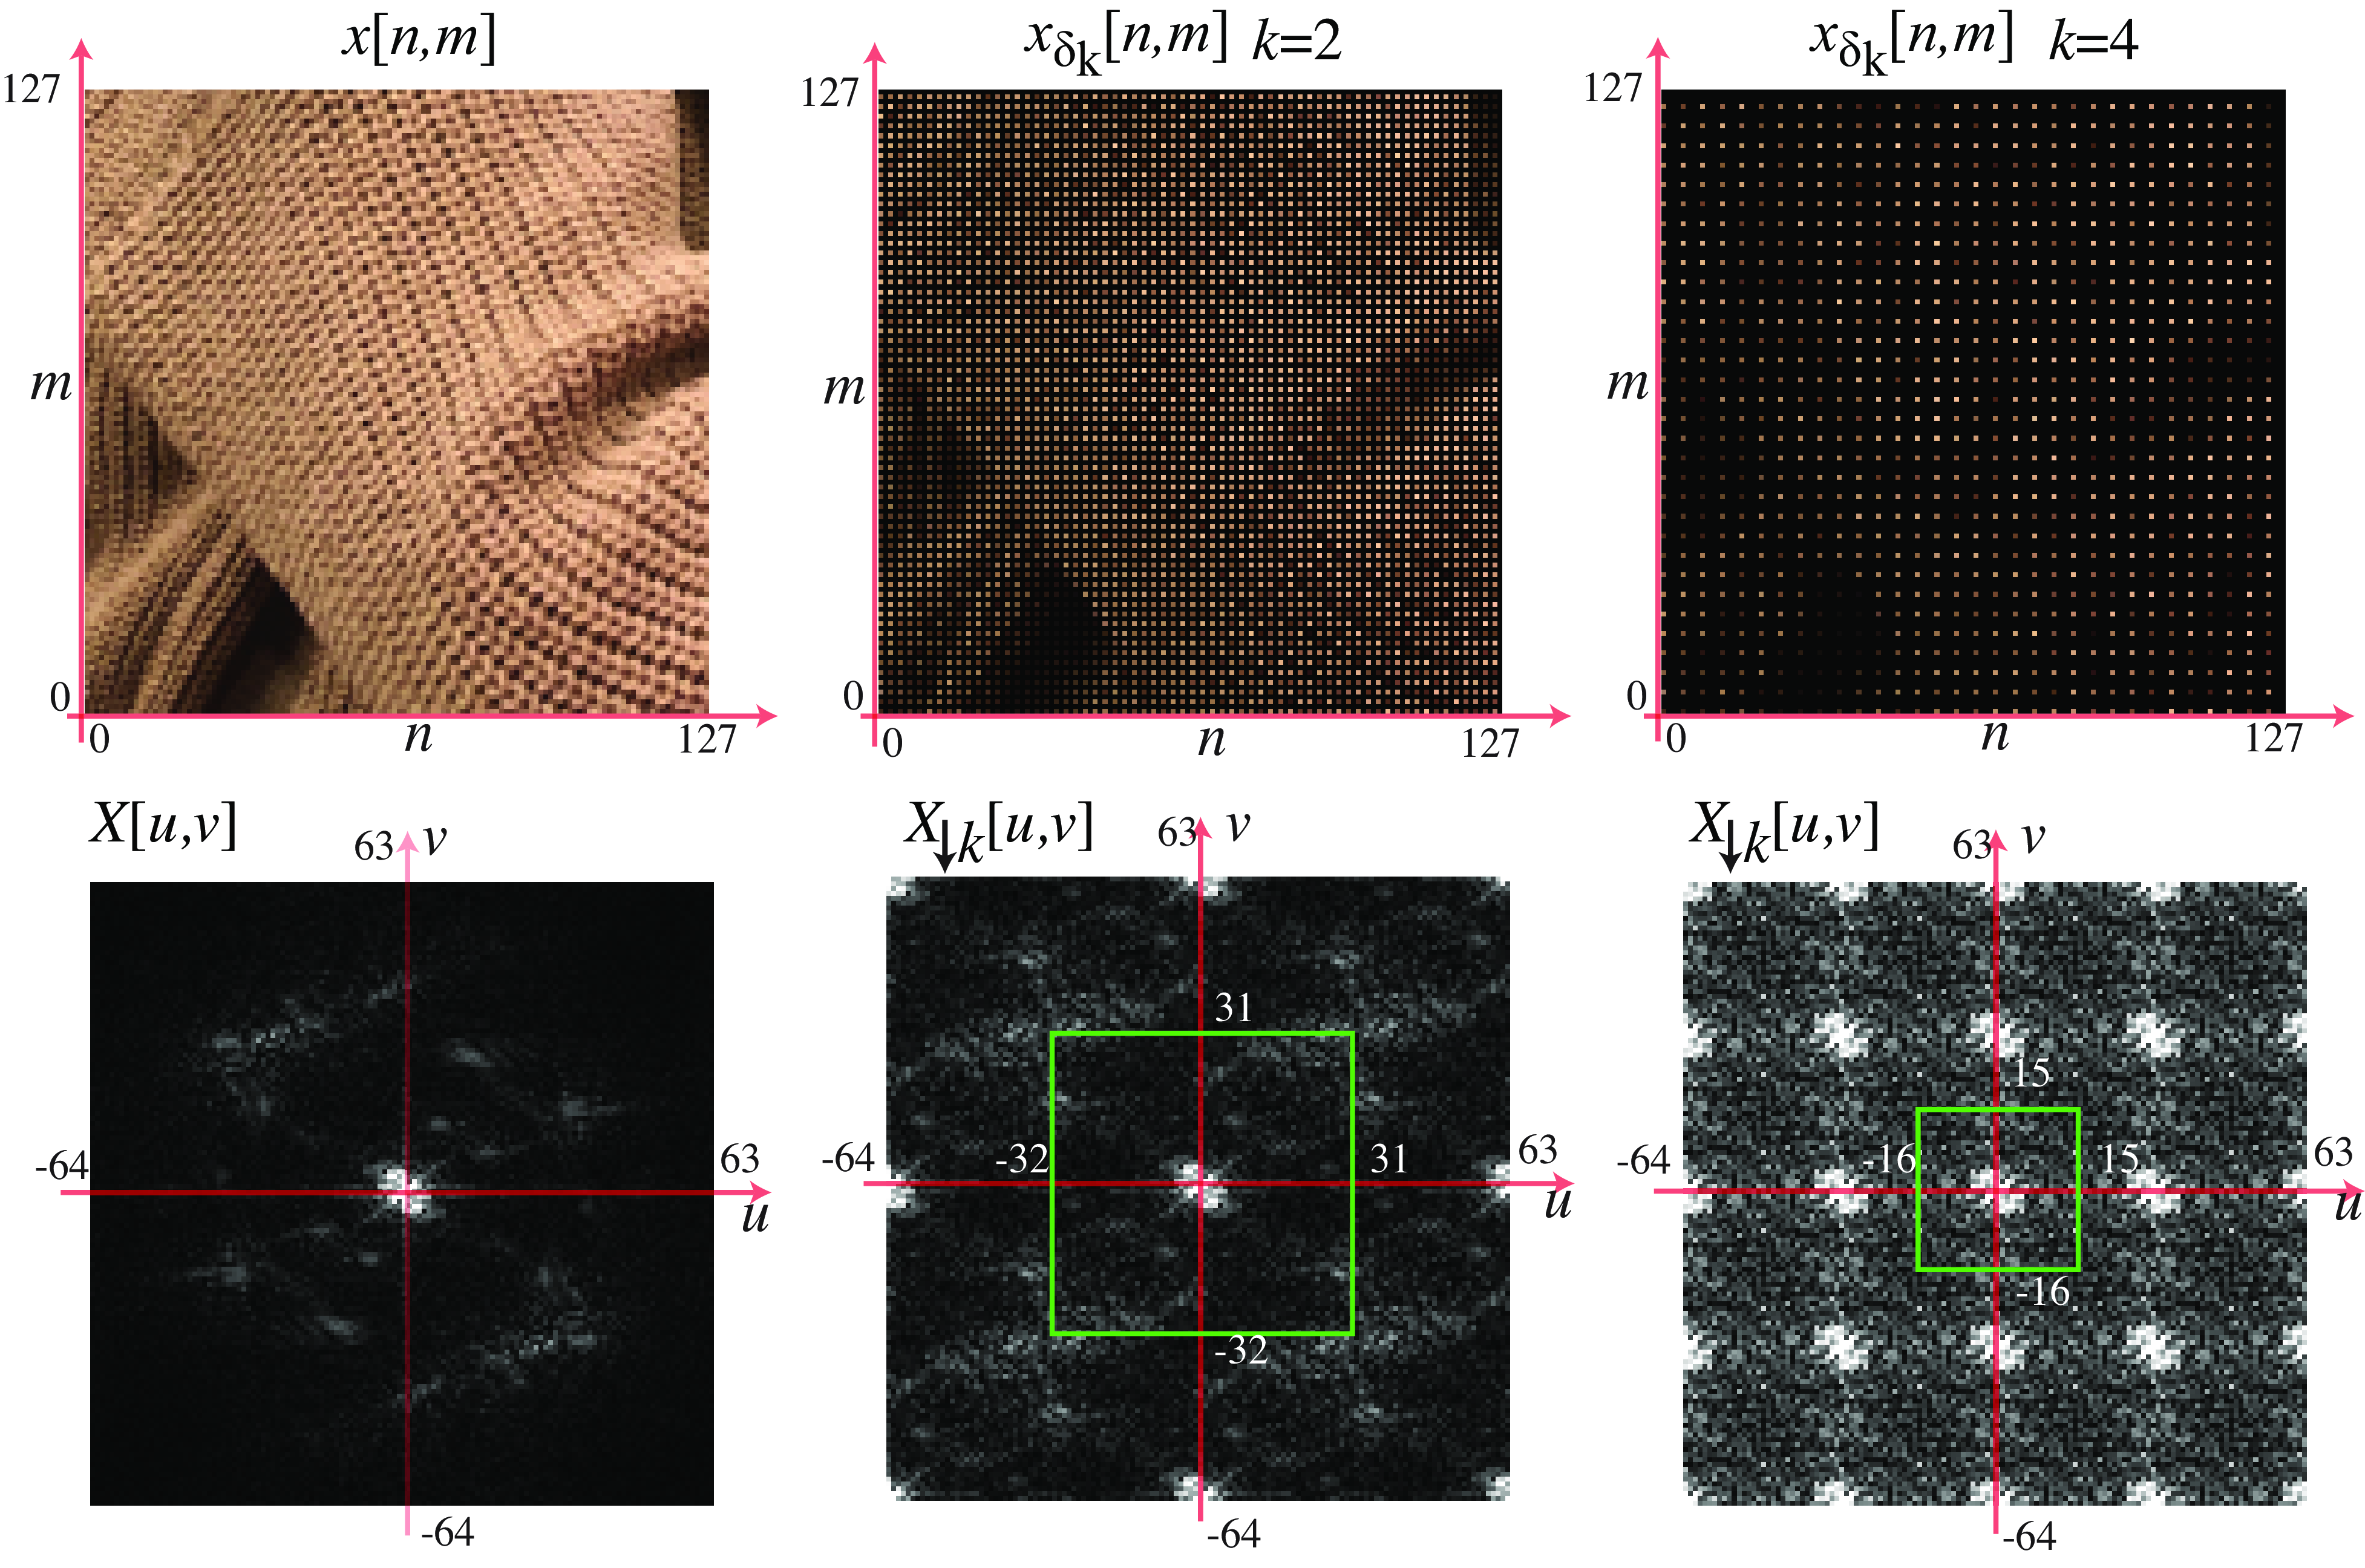
\includegraphics[width=1\linewidth]{figures/upsamplig_downsampling/discrete_texture_sampling.eps}
\end{center}

The resulting sampled images are (scaled so that they occupy the same area):

\begin{center}
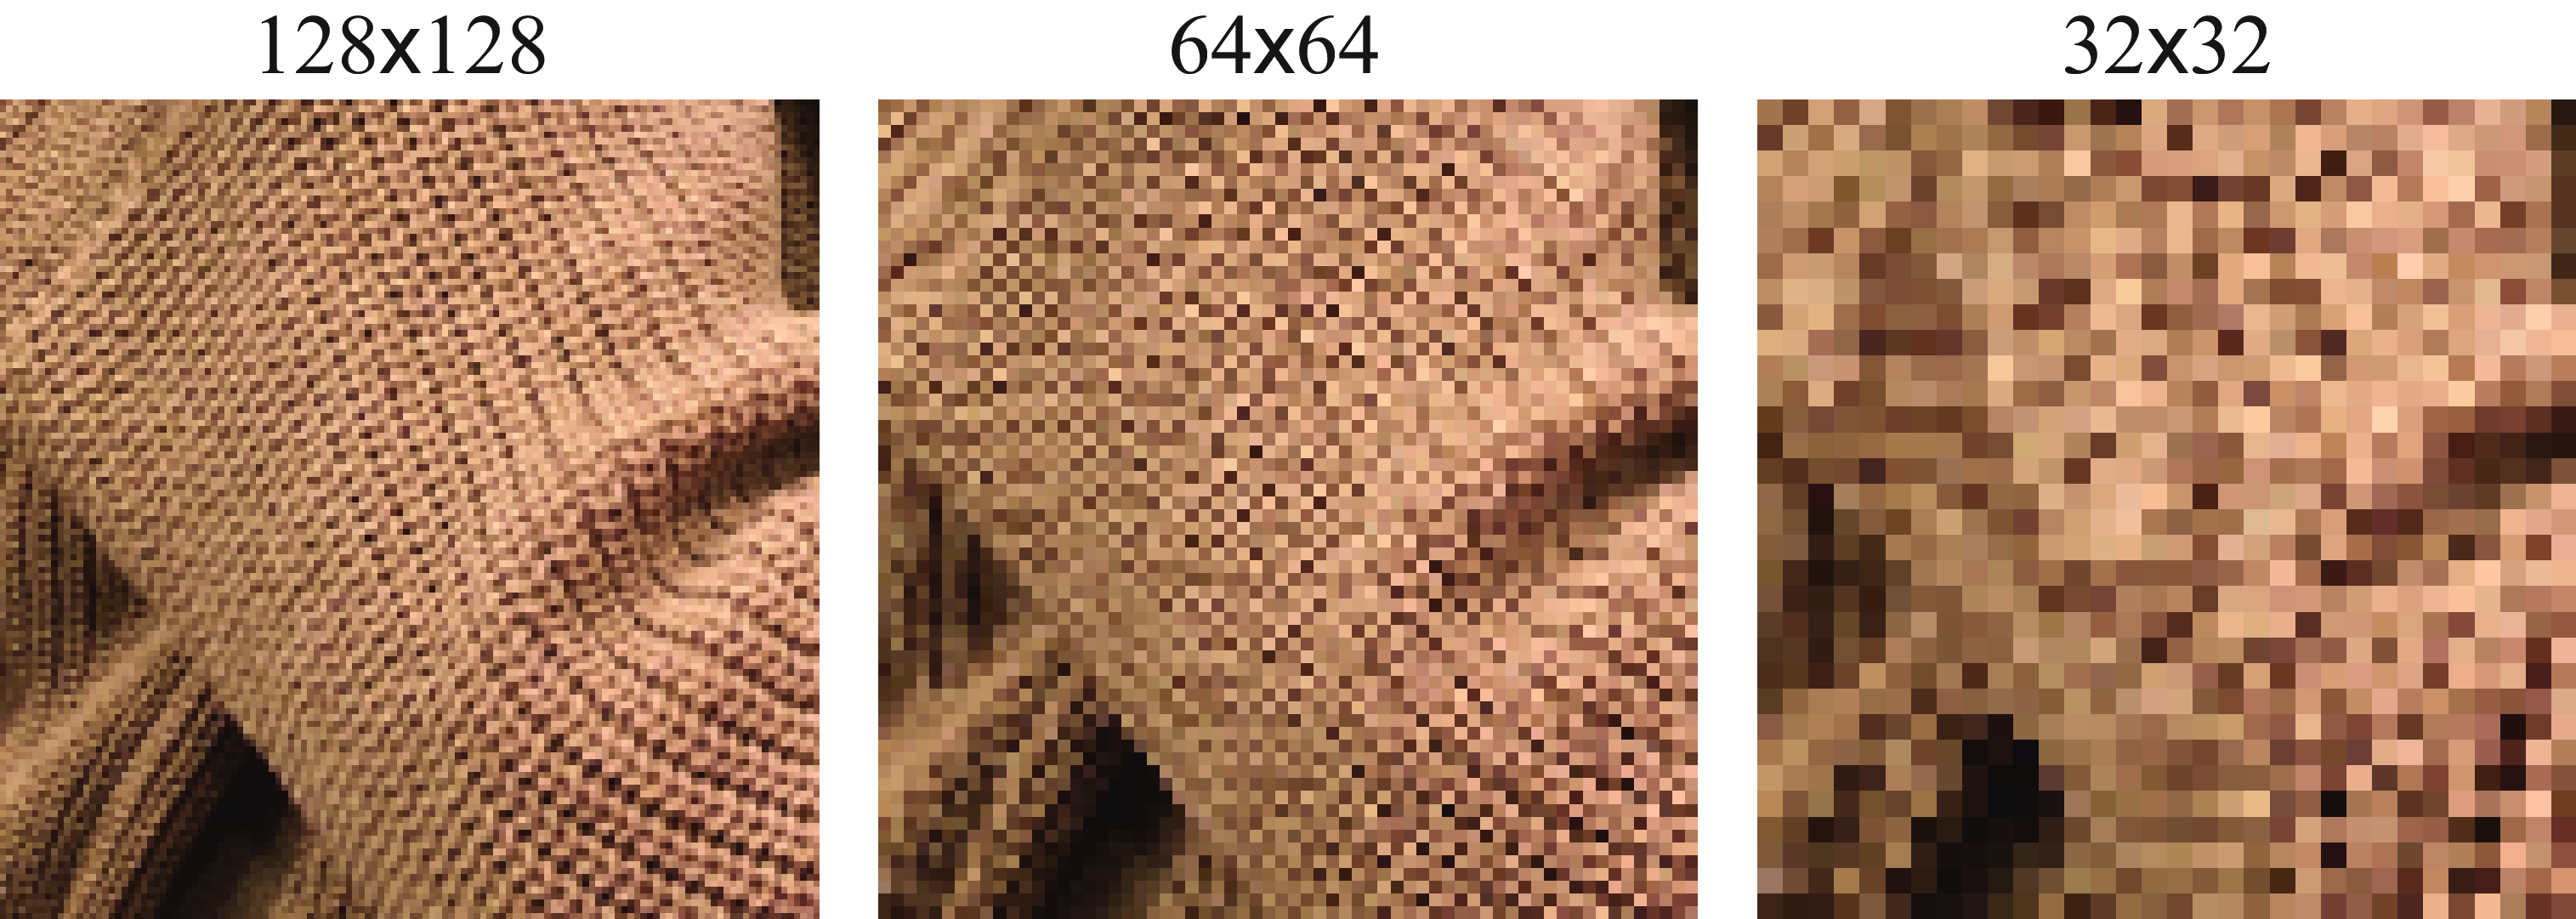
\includegraphics[width=1\linewidth]{figures/upsamplig_downsampling/subsampled_textures.eps}
\end{center}

As we downsample the image, we lose details in the texture such as the orientation of the knitting and it becomes harder to see the overall shape. Just reducing resolution by a factor of 4 results in an almost uninteligible image. The lost of information is both due to the reduced resolution, but most importantly, in this example, the aliasing. Aliasing has introduced new textural features in the subsampled image that are not present in the original image. 

How can we reduce the resolution of an image while preserving as much details as possible?


\subsection{Antialiasing filtering}

When sampling a signal of size $N \times N$ with a downsampling factor $k$, aliasing is produced by all the content at frequencies that are above $u,v > N/k$. We can remove content high spatial frequencies by using an antialiasing filter that will blur the image before downsampling.  

\begin{itemize}
\item Apply antialiasing filter: $g \left[ n,m \right] = f \left[n,m\right] \circ h_k \left[ n,m \right]$
\item Downsample the result:  $f_{\downarrow k} \left[n,m\right] = g\left[kn,km\right]$
\end{itemize}

One typical downsampling factor is $k=2$. In this case, we can apply the binomial filter on each dimension, $\left[1,2,1\right]/4 \circ \left[1,2,1\right]^T/4$, and then take one pixel every two (we apply a 1-pixel mirror boundary extension before applying the convolutions which we remove from the output). For efficiency, the antialiasing filter only needs to be computed on the samples that will be kept after downsampling. 




\begin{center}
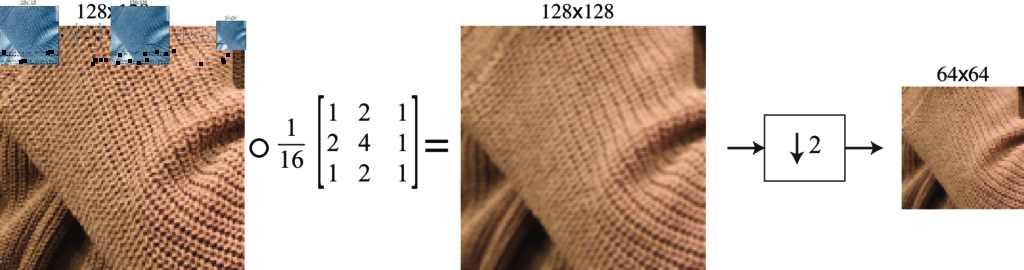
\includegraphics[width=1\linewidth]{figures/upsamplig_downsampling/downsampling_bilinear.eps}
\end{center}


In the anti-aliased downsampled images, fine details are gone while preserving the smooth details of the image. In fact, even at $32 \times 32$, we can still see some of the orientations of the knitting pattern and the shading due to the 3D shape.

\begin{center}
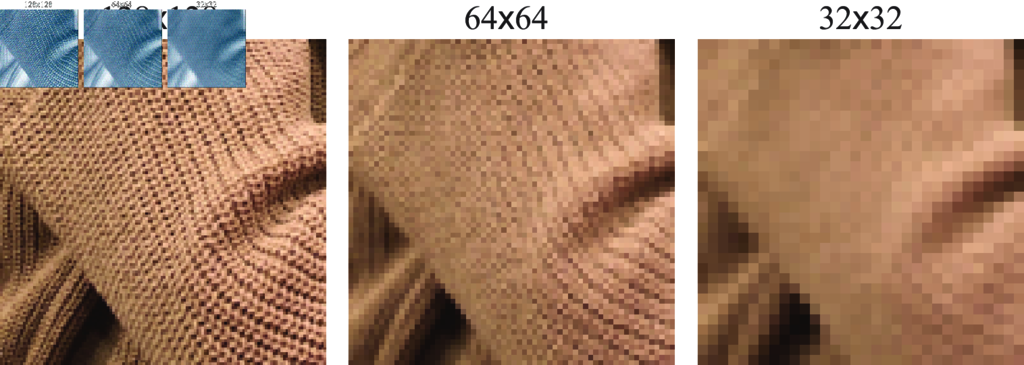
\includegraphics[width=1\linewidth]{figures/upsamplig_downsampling/subsampled_antialiasing_textures.eps}
\end{center}

Anti-aliansing is an essential operation whenever we manipulate the resolution of an image. 
As the convolution and downsampling are linear operators, sometimes it will be useful to write it as a matrix. For instance, for a 1D signal of length $N=6$  samples, if we downsample it by a factor $k=2$, then, using repeat padding for handling the boundary, and the binomial kernel as an antialiasing filter, we can write the downsampling operator as a matrix:
\begin{equation}
D = \left[ 
\begin{array}{cccccc}
3 & 1 & 0 & 0 & 0 & 0\\
0 & 1 & 2 & 1 & 0 & 0 \\
0 & 0 & 0 & 1 & 2 & 1  
\end{array}
\right]
\end{equation}



\section{Upsampling}

Upsampling consists in increasing the number of samples in the image. We will use the notation:
\begin{equation}
f_{\uparrow k} \left[n,m\right]  = f\left[n,m\right] \uparrow k 
\end{equation}

While downsampling is a well defined operator, upsampling requires increasing the resolution of an image from a low resolution image. This is a very challenging task as it requires recovering information that is not available on the low resolution image. The problem of making up new details will be called super-resolution and we will study it in chapter~\ref{}.  In this section we will focus on the simpler problem of creating an image that has $k \times k$ more pixels but that contains the same amount of information than the original low-resolution image. 

Upsampling consists in the next steps:
\begin{itemize}
\item Insert $k-1$ zeros between each sample on the horizontal dimension, and then on the vertical dimension. This will give us the image $\widehat{f}_k \left[n,m\right]$ of size $Nk \times Mk$:
\begin{equation}
\widehat{f}_k \left[n,m\right] = 
 \begin{cases}
    f \left[n/k,m/k\right]     & \quad \text{if } mod(n,k)=0 \text{~and~} mod(m,k)=0\\
    0       & \quad \text{otherwise }\\
  \end{cases}
  \label{eq:upzeros}
\end{equation}
\item Apply an interpolation filter: 
\begin{equation}
f_{\uparrow k} \left[n,m\right] = \widehat{f}_k \left[n,m\right] \circ h \left[n,m\right]
\label{eq:up_interp}
\end{equation}
\end{itemize}
Upsampling by a factor of two can also be done with two steps: 1) take the signal and insert one zero between each two samples (first for the horizontal dimension and then for the vertical one). 2) interpolate between samples applying the binomial filter $\left[1,2,1\right] \circ \left[1,2,1\right]^T$. You need to divide the result by 4 to get the same range of intensity values as the input. The convolution (eq.~\ref{eq:up_interp}) only needs to be computed on the samples to be interpolated. In this example, you could convolve the rows of the original image with the filter $\left[1,1\right]/2$ and then create a new signal taking one pixel from the original image and one pixel from the result of this convolution. Then repeat the same operation with the columns. Note that upsampling uses a low resolution version of the input signal to increase the amount of samples! This is certainly something very different to super-resolution where we want to create an image that looks sharper. 


\begin{figure}
\includegraphics[width=1\linewidth]{figures/upsamplig_downsampling/upsampling_bilinear.eps}
\caption{Upsampling by a factor of $k=2$ using a bilinear interpolation filter. The top row shows the images and the bottom row shows the magnitude of their DFTs. Note that the filter does not suppress completely the copies of the original DFT that appear when inserting new samples. Remember that the DFTs have the same number of samples as the corresponding input image. The DFT of the kernel is shown by zero padding the convolutional kernel to match the image size. The ideal filter is a box filter with the support defined by the green square.  However, the interpolated image looks reasonably good.
} 
\label{fig:upsamplingazebra}
\end{figure}

Figure.~\ref{fig:upsamplingazebra} shows the upsampling process for a color image. Each color channel is upsampled by a factor of $k=2$ independently. 

The binomial filter is not the best interpolation filter, but it is very efficient. But when quality is important, there are better interpolation filters.  The following list details the most commonly used interpolation filters. All interpolation filters are separable, so they can be written as $h\left[n,m\right] = h\left[n\right] h\left[m\right]$:
\begin{itemize}
\item Nearest neighbor interpolation: assign to each interpolated sample the value of the closest sample. This can be done by convolving the image from eq.~\ref{eq:upzeros} with the kernel (if $k$ is even):
\begin{equation}
h  \left[n\right] =  \begin{cases}
    1     & \quad \text{if }  n \in  \left[-k/2, k/2\right] \\
    0       & \quad \text{otherwise }\\
\end{cases}
\end{equation}
this is very fast as it only requires replicating samples. But it gives very low quality. 

\item Bilinear interpolation: for each row linearly interpolate each sample with the two nearest neighbors. Then do the same for the columns. This can also be written as a convolution with the kernel (if $k$ is even):
\begin{equation}
h  \left[n\right] =  \begin{cases}
    (k-n)/k     & \quad \text{if }  n \in \left[-k/2, k/2\right] \\
    0       & \quad \text{otherwise }\\
\end{cases}
\end{equation}
It is a triangular separable kernel. Note that for $k=2$, the bilinear interpolation in 2D is the $3 \times 3$ kernel: $\left[1/2,1,1/2\right] \circ \left[1/2,1,1/2\right]^T$.

\item Bicubic interpolation:

\item Lanczos interpolation:

\item Ideal interpolation:

\end{itemize}

The upsampling operator is also a linear operation, therefore we can also write it in matrix form. For instance, for a 1D signal of length $N=3$  samples, if we upsample it by a factor $k=2$, then, using repeat padding for handling the boundary and the bilinear interpolation, then we can write the upsampling operator as a matrix:
\begin{equation}
U = \left[ 
\begin{array}{ccc}
1    & 0    & 0 \\
0.5 & 0.5 & 0 \\
0    & 1    & 0 \\
0    & 0.5 & 0.5 \\
0    & 0    & 1 \\
0    & 0    & 1 
\end{array}
\right]
\end{equation}
Multiplying this matrix by a signal of length 3, gives an output of length 6. Samples 1, 3 and 5 are copies of the input, while samples 2 and 4 are computed as the average of two input samples. The last output is a copy of the last input sample because it corresponds to extending the input using repeat padding.


\section{Translation invariance and the importance of anti-aliasing filtering}


\section{Discussion}


